\documentclass{article}
\usepackage{amsmath}
\usepackage{amssymb}
\usepackage{graphicx}
\author{Yichen ZHU}
\title{Compte rendu TP Localisation}
\begin{document}
\maketitle

\section{Localisation avec ancres}
\paragraph{} On veut conna\^itre la position d'un capteur $(\theta=(x,y))$ \`a partir des $M$ ancres autour du capteur $[z_{1}=(\alpha_{1},\beta_{1}) \cdots z_{M}=(\alpha_{M},\beta_{M})]$. On conna\^it toutes les distances entre les ancres et le capteurs $(d_{1} \cdots d_{M})$ On a donc :
\begin{align*}
d^{2}_{k} &= \left\|\theta-z_{k}\right\|^{2} \\
          &= \left\|\theta\right\|^{2} - 2\left\langle z_{k},\theta\right\rangle + \left\|z_{k}\right\|^{2}\\
\intertext{Pour $k$ allant de 2 \`a M}
d^{2}_{k} - d^{2}_{1} &= -2\left\langle z_{k}-z_{1},\theta\right\rangle + \left\|z_{k}\right\|^{2} - \left\|z_{1}\right\|^{2} \\
											&= -2\left\langle z_{k}-z_{1},\theta\right\rangle + (\alpha^{2}_{k}-\alpha^{2}_{1}+\beta^{2}_{k}-\beta_{1})
\end{align*}
On peut r\'esumer cette relation par : 
\[
\Phi\theta = b - \delta
\]
avec $\Phi = 2\begin{pmatrix}                               
								\alpha_{2}-\alpha_{1} & \beta_{2}-\beta_{1} \\
								\vdots         &        \vdots \\
								\alpha_{M}-\alpha_{1} & \beta_{M}-\beta_{1} \\
							\end{pmatrix}$
			$b = \begin{pmatrix}	
						\alpha^{2}_{2}-\alpha^{2}_{1}+\beta^{2}_{2}-\beta_{1} \\
						\vdots \\
						\alpha^{2}_{M}-\alpha^{2}_{1}+\beta^{2}_{M}-\beta_{1}
					\end{pmatrix}$
			$\delta = \begin{pmatrix}
								 d^{2}_{2} - d^{2}_{1} \\
								 \vdots \\
								 d^{2}_{M} - d^{2}_{1}
							 \end{pmatrix}$
En observation, on mesure les puissances autour des ancres avec un bruit pour estimer les distances. Une fois on a les distances estim\'ees	$(\widehat{d}^{2}_{1} \cdots \widehat{d}^{2}_{M})$ on a notre $\widehat{\delta}$ d'o\`u on \'etablit la nouvelle \'equation :
\[
\Phi\theta = b - \widehat{\delta}
\]
On cherche le $\theta$ qui satisfait toutes \'equations pour $k$ allant de 2 \`a $M$ mais on ne peut pas le r\'esoudre parce que avec $M$ \'equations, deux inconnus, la solution n'est pas unique. On veut donc estimer $\theta$ au sens moindre-carr\'es c'est \`a dire on cherche un $\theta$ qui minimise : $\left\|\Phi\theta - (b - \widehat{\delta})\right\|^{2}$. Donc : 
\begin{align*}
\widehat{\theta} &= \operatorname{arg\,min}_\theta \left\|\Phi\theta - (b - \widehat{\delta})\right\|^{2} \\
\intertext{On calcule le gradient}
               0 &= \nabla_{\theta}(\left\|\Phi\theta - (b - \widehat{\delta})\right\|^{2}) \\
							   &= \Phi^{T}(\Phi\theta-(b - \widehat{\delta})) \\
\Rightarrow 
\Phi^{T}\Phi\widehat{\theta} &= \Phi^{T}(b-\widehat{\delta}) \\
						\widehat{\theta} &= (\Phi^{T}\Phi)^{-1}\Phi^{T}(b-\widehat{\delta})
\end{align*} 
\paragraph{} On impl\'emente cette m\'ethode en Matlab et on joue avec les param\`etres M (nombre d'ancres) et T (nombre de mesures) :
\begin{figure}[h]
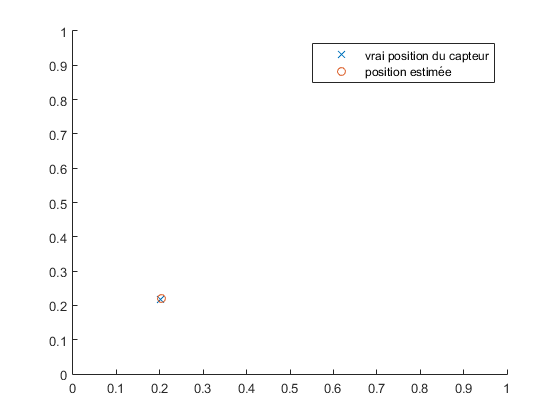
\includegraphics[scale=0.4]{ancre_M5T100.png} 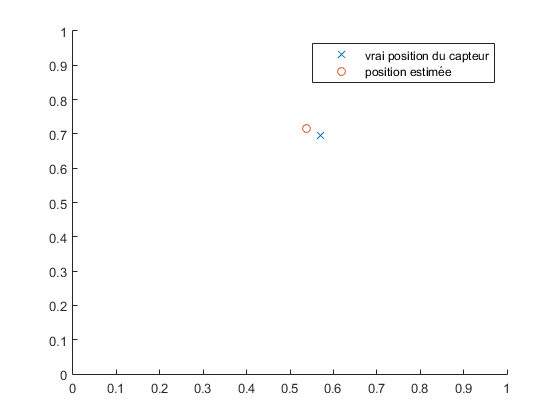
\includegraphics[scale=0.4]{ancre_M5T10.png} 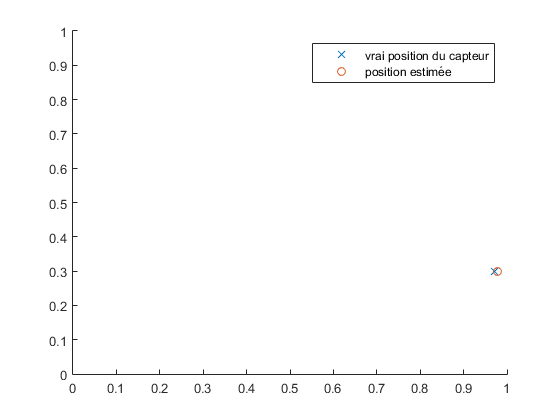
\includegraphics[scale=0.4]{ancre_M10T10.png} 
\caption{$M=5$ $T=100$, $M=5$ $T=10$ et $M=10$ $T=10$}
\end{figure} 
\\On remarque quand on a plus d'ancres ou plus de mesures par ancres, l'estimation est plus pr\'ecise.
\paragraph{} Maintenant on s'int\'eresse \`a un autre estimateur au sens du maximum de vraisemblance. \`A partir des observations des puissances, on veut chercher un $\widehat{\theta}$ qui minimise les erreurs $E =\frac{(P_{0}-\overline{P})}{10(\eta-\log_10 (\widehat{\theta}-z/d_{0}))}$ On peut effectuer une approximation avec l'algorithme du gradient stochastique :
\[
\widehat{\theta}_{n+1} = \widehat{\theta}_{n} + \gamma\overline{E*(\widehat{\theta}_{n}-z)/\left|\widehat{\theta}_{n}-z\right|^{2}}
\]
On impl\'emente cet algorithme et on compare les r\'esultats pour les diff\'erentes valeurs du pas $\gamma$.
\begin{figure}[!h]
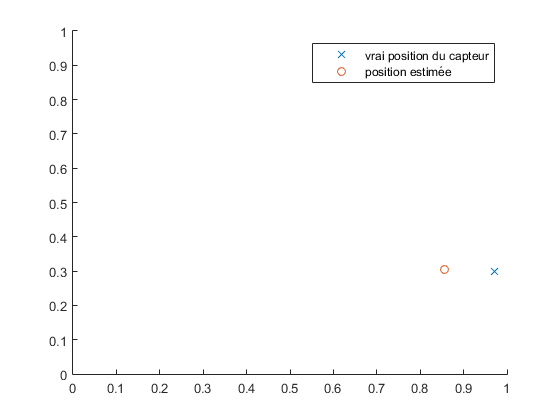
\includegraphics[scale=0.35]{grad_gamma0002.png} 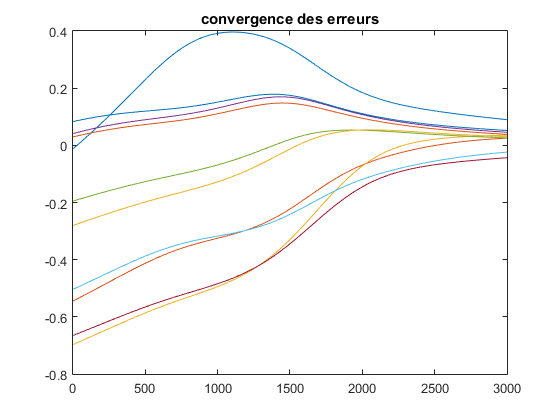
\includegraphics[scale=0.35]{grad_err_gamma0002.png} 
\caption{$\gamma=0.002$}
\end{figure} 
\begin{figure}[!h]
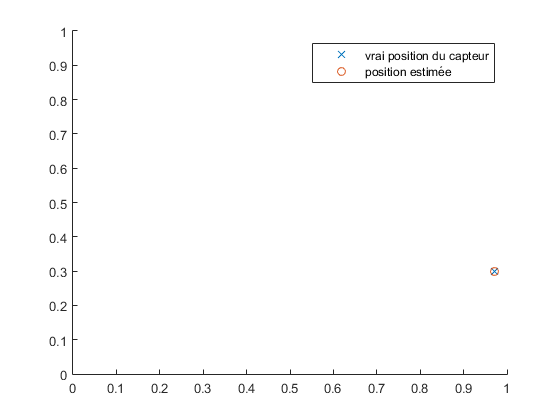
\includegraphics[scale=0.35]{grad_gamma001.png} 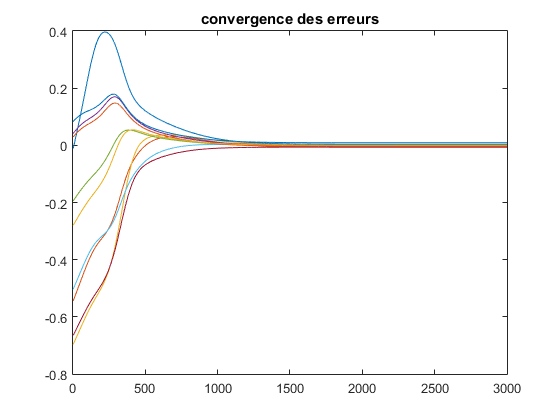
\includegraphics[scale=0.35]{grad_err_gamma001.png} 
\caption{$\gamma=0.01$}
\end{figure} 
\begin{figure}[!h]
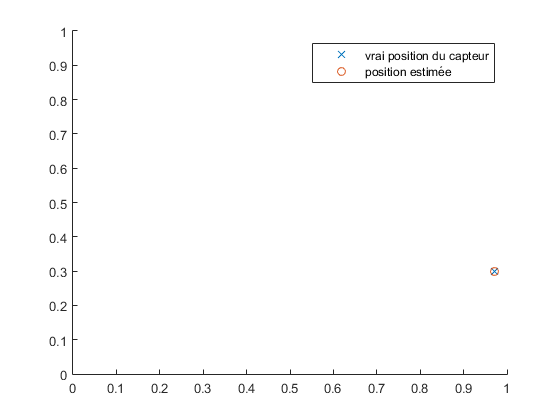
\includegraphics[scale=0.35]{grad_gamma01.png} 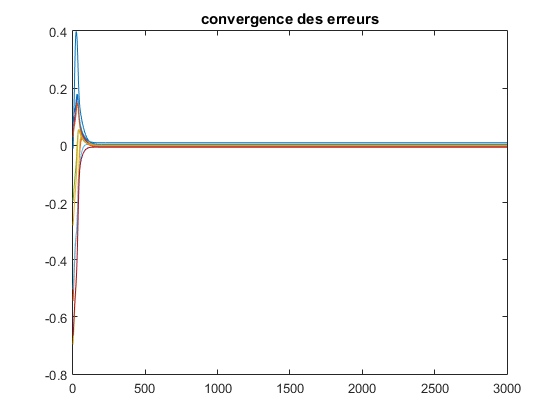
\includegraphics[scale=0.35]{grad_err_gamma01.png} 
\caption{$\gamma=0.1$}
\end{figure} 
\\On peut voir quand on augmente le pas, l'algorithme converge plus vite. On arrive toujours \`a bien localiser le capteur si le nombre d'it\'eration est suffisant pour que l'algorithme converge. Par rapport \`a la m\'ethode de moindre carr\'es, on arrive tous \`a localiser le capteur et la performance d\'epend de la quantit\'e de donn\'ees. Si on a peu d'ancres et peu de nombre de mesures par ancre, on utiliserai la m\'ethode du gradient stochastique et en revanche quand chaque ancre mesure plusieurs fois, il vaut mieux de prendre la m\'ethode de moindre carr\'es parce que la complexit\'e de la m\'ethode du gradient est plus grande.
\\
\paragraph{} Maintenant on fait d\'eplacer le capteur et on veut estimer sa position en ligne avec une m\'ethode adaptative. On cherche \`a minimiser $\mathbb{E}(\left\|\Phi\theta - (b - \widehat{\delta}_{n})\right\|^{2})$.
On montre d'abord que : $\mathbb{E}[\left\|\Phi\theta - (b - \widehat{\delta}_{n})\right\|^{2}] = \left\|\Phi\theta - (b - \delta)\right\|^{2} $
\begin{align*}
\mathbb{E}[\left\|\Phi\theta - (b - \widehat{\delta}_{n})\right\|^{2}] &= \mathbb{E}[\left\|\Phi\theta\right\|^{2}-2\left\langle b-\widehat{\delta}_{n},\theta\right\rangle] + Cst \\
          &= \left\|\Phi\theta\right\|^{2} -2\left\langle b-\mathbb{E}(\widehat{\delta}_{n}),\theta\right\rangle + Cst \\
					\intertext{On a $\mathbb{E}(\widehat{\delta}_{n})=\mathbb{E}(\delta)$}
					&= \left\|\Phi\theta\right\|^{2} -2\left\langle b-\delta,\theta\right\rangle + Cst \\
					&= \left\|\Phi\theta - (b - \delta)\right\|^{2} 
\end{align*}
Le probl\`eme de minimisation devient donc : $\operatorname{arg\,min}_\theta \mathbb{E}[\left\|\Phi\theta - (b - \widehat{\delta}_{n})\right\|^{2}] $
On peut donc conclure l'algorithme de LMS :
\begin{align*}
\widehat{\theta}_{n+1} &= \widehat{\theta}_{n} - \gamma\nabla_{\theta}(\left\|\Phi\theta - (b - \widehat{\delta})\right\|^{2}) \\
											 &= \widehat{\theta}_{n} - \gamma\Phi^{T}(\Phi\widehat{\theta}_{n} - (b-\widehat{\delta}_{n+1})) \\
\end{align*}

En pratique, on impl\'emente l'algorithme LMS et on modifie les param\`etres pas et bruit pour voir l'influence. On fait d'abord v\'erifier le pas :
\begin{figure}[h]
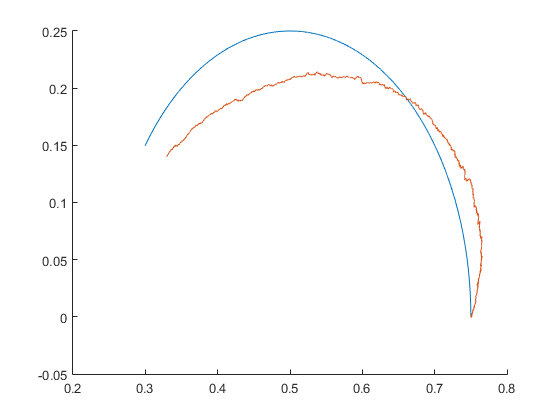
\includegraphics[scale=0.25]{LMS_gamma0005.png} 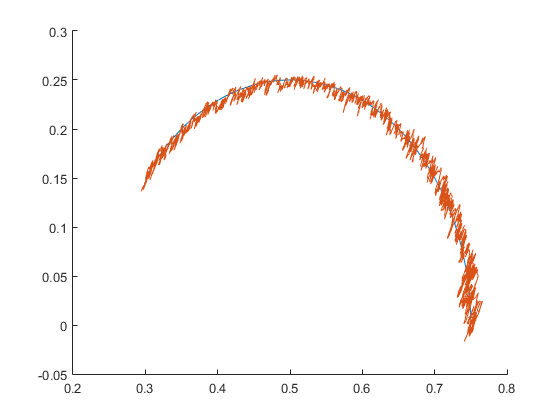
\includegraphics[scale=0.25]{LMS_gamma005.png} 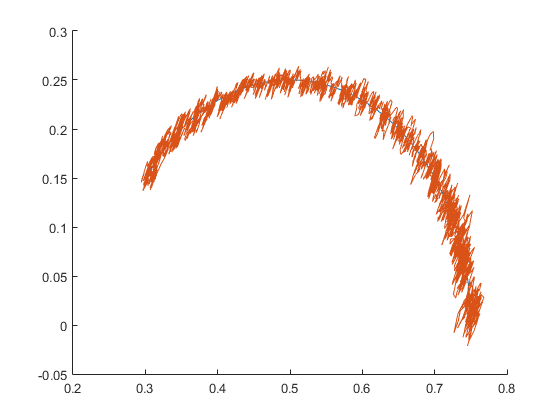
\includegraphics[scale=0.25]{LMS_gamma01.png} 
\caption{$\gamma=0.005$, $\gamma=0.05$ et $\gamma=0.1$}
\end{figure} 
\\On peut conclure que le choix du pas est un jeu de compromis entre la transitoire et la fluctuation. Quand $\gamma$ est petit, la fluctuation est petite mais la transitoire est trop lente pour suivre le capteur. Quand on fait augmenter le $\gamma$, l'observation arrive \`a suivre la trajectoire mais le niveau du bruit est plus pr\'esent.

Ensuite, on fait varier le bruit $\sigma$ et on voit que cela n'influe que sur la partie fluctuation.
\begin{figure}[h]
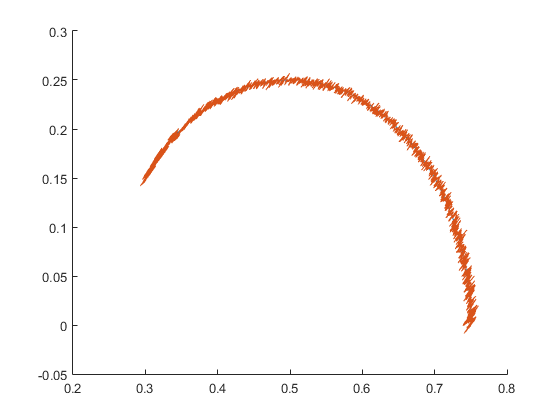
\includegraphics[scale=0.4]{LMS_sigma001.png} 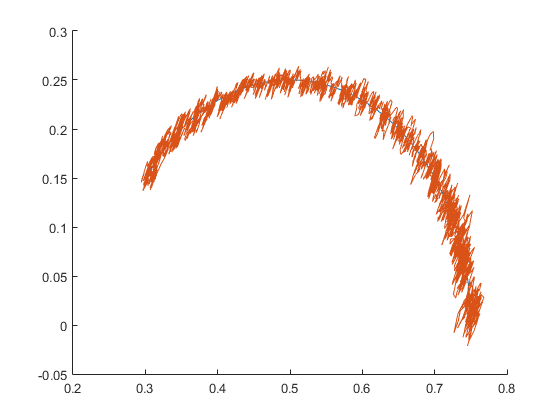
\includegraphics[scale=0.4]{LMS_gamma01.png} 
\caption{$\gamma=0.1$ $\sigma=0.1$ et $\gamma=0.1$ $\sigma=0.3$}
\end{figure} 

\section{Localisation sans ancres}
On va localiser plusieurs capteurs sans ancres. On mesures les distances inter-capteurs. On ne peut r\'ecup\'erer les positions qu'\`a une isom\'etrie pr\`es parce qu'on n'a aucune donn\'ee absolue dans le plan. 
\\Ensuite, on g\'en\`ere les capteurs dans le plan :
\begin{center}
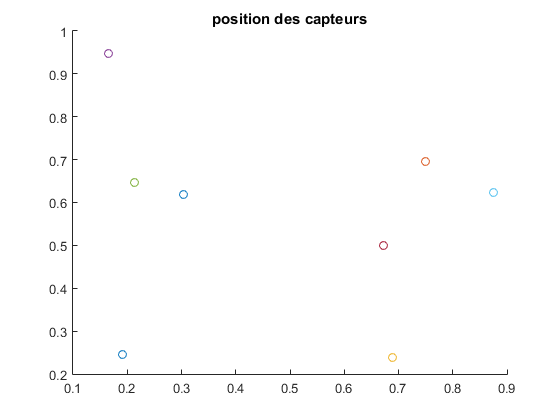
\includegraphics[scale=0.5]{sans_ancres1.png}
\end{center}
On g\'en\`ere la matrice qui contient toutes les distances inter-capteurs :
\[
D = \begin{pmatrix}
			0 & d^{2}_{1,2} & d^{2}_{1,3} & \cdots & d^{2}_{1,N} \\
      d^{2}_{2,1} & 0 & d^{2}_{2,3} & \cdots & d^{2}_{2,N} \\
		  d^{2}_{3,1} & d^{2}_{3,2} & 0 & \cdots & d^{2}_{3,N} \\
			\vdots & \vdots & \vdots & \ddots & \vdots \\
			d^{2}_{N,1} & \cdots & -\frac{1}{N} & \cdots & 0
	  \end{pmatrix}
\]
\\et on a $P = \begin{pmatrix}
								1-\frac{1}{N} & -\frac{1}{N} & \cdots & -\frac{1}{N} \\
								-\frac{1}{N} & 1-\frac{1}{N} & \ddots & \vdots\\
								\vdots & \ddots & 1-\frac{1}{N} & -\frac{1}{N} \\
								-\frac{1}{N} & \cdots & -\frac{1}{N} & 1-\frac{1}{N}
						 \end{pmatrix}$ et $M = -\frac{1}{2}PDP$
\\En prenant les deux valeurs propres qui sont non-nulles et les vecteurs associ\'es de la matrice $M$, on trace dans le plan les coordonn\'ees $(\sqrt{\lambda_{1}}\nu_{1},\sqrt{\lambda_{2}}\nu_{2})$ :
\begin{center}
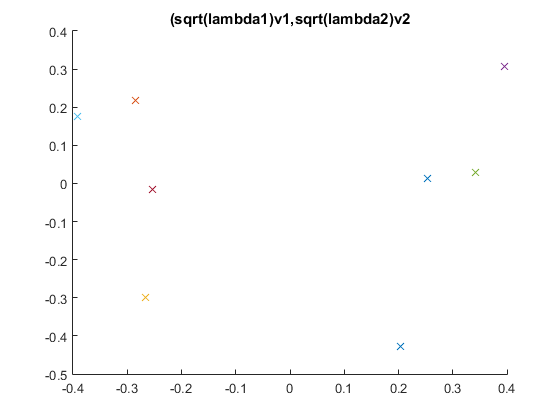
\includegraphics[scale=0.5]{sans_ancres2.png}
\end{center}
On remarque que les distances inter-capteurs sont les m\^emes. On pourrais faire l'estimation en retirant les valeurs et vecteurs propres de la matrice $M$.

On veut montrer th\'eoriquement : $M = ZZ^{T}$. Le principe est de d\'evelopper $PDP$ et voir si c'est \'egal \`a $-2ZZ^{T}$.

On fait maintenant la localisation en ligne en appliquant l'algorithme d'Oja. On fait d\'eplacer les capteurs comme pr\'ec\'edemment :
\begin{center}
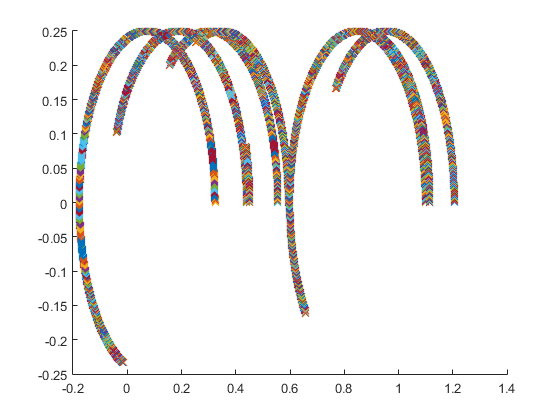
\includegraphics[scale=0.5]{oja.png}
\end{center}
Ici on ne peut pas avoir des points estim\'es qui suivent la trajectoire parce qu'on ne peut pas r\'ecup\'erer des positions absolues. Le seul
moyen de v\'erifier le fonctionnement de l'algorithme est de voir \`a tel instant, les distances inter-capteurs sont \`a peu pr\`es pareils.
On a ci-dessous $n=4000$ et	$n=5000$ :
\begin{figure}[h]
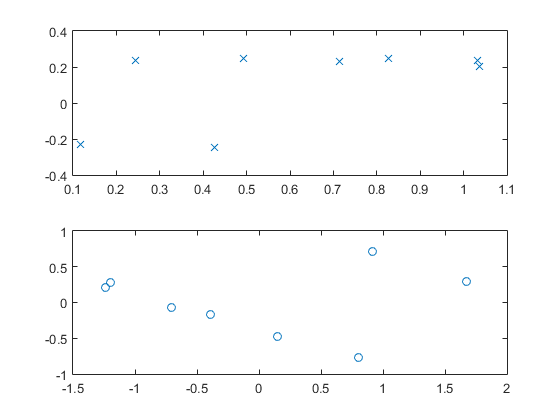
\includegraphics[scale=0.4]{sans_ancres_oja.png} 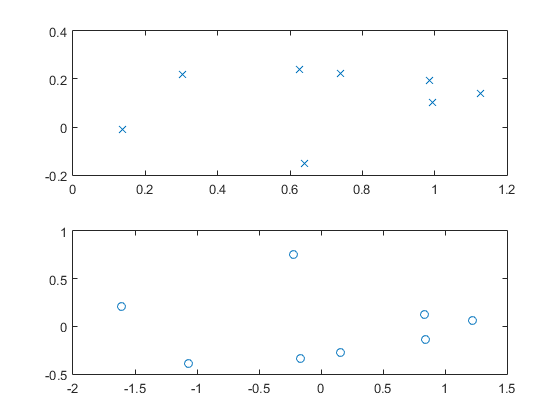
\includegraphics[scale=0.4]{sans_ancres_oja2.png} 
\caption{$n = 4000$, $n=5000$}
\end{figure} 
\\On remarque les vraies capteurs et ceux estim\'es ont la m\^eme forme. L'un peut \^etre obtenu par l'autre avec soit la rotation soit le mirroir. Cela v\'erifie le bon fonctionnement de l'algorithme. Comme cela est aussi un algorithme adaptatif, le choix du pas est comme l'algorithme de LMS qu'on a vu pr\'ec\'edemment, on veut avoir un compromis entre la transitoire et la fluctuation. 
											
\end{document}